\documentclass{beamer}
\usepackage[utf-8]{inputenc}
\usepackage{graphicx, subfigure}
\usepackage{longtable}
\usepackage{amsmath,amsfonts}
\usepackage{array}
\usepackage{xspace}
\usepackage{color, fancyvrb, relsize}
\usepackage{url, hyperref}
\usepackage{algorithm, algorithmic, listings}
\usepackage[francais]{babel}
\selectlanguage{francais}

\newcommand{\<}[1]{\`#1}

%ref: http://tex.dante.jp/typo/index.php?Listings#l8795a28

\usepackage{color,graphicx}
%\usepackage[margin=2.5cm]{geometry}
%\usepackage{type1cm}
\usepackage{listings}

\lstdefinelanguage{Scheme}{%
   keywords={begin,call-with-current-continuation,call/cc,%
      call-with-input-file,call-with-output-file,case,cond,do,%
      delay,else,force,for-each,if,lambda,let,let-syntax,let*,%
      letrec,letrec-syntax,and,or,not,map,syntax,syntax-rules,%
      with-mode,with-input-from-file,with-input-fromport,%
      with-output-to-file,with-output-to-port,define,%
			set!, eq?, equal?, eqv?, symbol?, string?, string=?,
			append, string-append, vector-append, string, vector,
			symbol, symbol->string, string->symbol, list, list-ref,
			list-set!, list-tail, set-car!, set-cdr!, car, cdr,
			vector-ref, vector-set!
   },%
   sensitive,%
   alsodigit=-,%
   morecomment=[l]{;},% 
   morecomment=[s]{\#|}{|\#},% 
   morestring=[b]{"}% 
  }[keywords,comments,strings]%"

\lstdefinelanguage[MIT]{Scheme}{%
   morekeywords=[1]{begin,call-with-current-continuation,call/cc,%
      call-with-input-file,call-with-output-file,case,cond,do,%
      delay,else,force,for-each,if,lambda,let,let-syntax,let*,%
      letrec,letrec-syntax,and,or,not,map,syntax,syntax-rules,%
      with-mode,with-input-from-file,with-input-fromport,%
      with-output-to-file,with-output-to-port,define%
   },%
   morekeywords=[2]{fluid-let,%
     in-package,local-declare,macro,make-environment,named-lambda,%
     using-syntax,with-input-from-string,with-output-to-string,%
     with-values,syntax-table-define,list-transform-positive,%
     list-transform-negative,list-search-positive,list-search-negative,%
     access-components,assignment-components,combination-components,%
     comment-components,conditional-components,disjunction-components,%
     declaration-components,definition-components,delay-components,%
     in-package-components,lambda-components,lambda-components*,%
     lambda-components**,open-block-components,pathname-components,%
     procedure-components,sequence-components,unassigned?-components,%
     unbound?-components,variable-components,%
     \#t,\#f,\#e,\#i,\#b,\#o,\#d,\#l,\#s,\#x,\#!\#*,\#@,\#=,\#\#,%
     access,cons-stream,declare,default-object?,define-integrable,%
     define-structure,define-syntax,er-macro-transformer,%
     non-hygienic-macro-transformer,quasiquote,quote,%
     rsc-macro-transformer,sc-macro-transformer,set!,%
     eq?,eqv?,equal?,%
     gcd,modulo,imag-part,numerator,inexact->exact,quotient,abs,%
     lcm,rationalize,angle,magnitude,real-part,ceiling,make-polar,%
     remainder,denominator,make-rectangular,round,expt,max,truncate,%
     floor,min%
  }%
   sensitive=true,%
   alsodigit=-,%
   morecomment=[l]{;},% 
   morecomment=[s]{\#|}{|\#},% 
   morestring=[b]{"}% "
}

\lstset{%
 frame=single,%
 keywordstyle={\ttfamily \color[rgb]{.1, .7, .7}},%
 stringstyle={\ttfamily \color[rgb]{0,.9,0}},%
 commentstyle={\ttfamily \color[rgb]{.9,0,0}},%
 identifierstyle={\color[rgb]{0,0,0}},%
 basicstyle={\ttfamily \color[rgb]{0,0,0}},%
 breaklines=true,%
 columns=[l]{fullflexible},%
 numbers=left,%
 %stepnumber=5,%
 numberstyle={\scriptsize},%
 numbersep=1em,%
 language={Scheme},%
}
\newcommand*\schemesrc[1]{\lstinputlisting[caption={question~#1}]{#1.scm}}



\lstloadlanguages{C,Haskell,Prolog,ML,Lisp,Scheme}
\lstset{language=Scheme}
\lstset{moredelim=*[is][\ttfamily \color{blue}]{|-}{-|}}
%\lstset{moredelim=*[s][\color{red}]{(}{\ }}}

% for themes, etc.
\mode<presentation>
{ \usetheme{boxes} }

\usepackage{times}  % fonts are up to you
\usepackage{graphicx}

% these will be used later in the title page
\title{Développement de Space Invaders}
\author{David St-Hilaire}
\titlegraphic{\includegraphics[scale=0.7]{medium-intro}}

\date{Juin 2008}

% note: do NOT include a \maketitle line; also note that this title
% material goes BEFORE the \begin{document}

% have this if you'd like a recurring outline
\AtBeginSection[]  % "Beamer, do the following at the start of every section"
{
\begin{frame}<beamer> 
\frametitle{Outline} % make a frame titled "Outline"
\tableofcontents[currentsection]  % show TOC and highlight current section
\end{frame}
}

\begin{document}

% this prints title, author etc. info from above
\begin{frame}
\titlepage
\end{frame}

%%%%%%%%%%%%%%%%%%%%%%%%%%%%%%%%%%%%%%%%%%%%%%%%%%%%%%%%%%%%%%%%%%%%%%%%%%%%%%%

\section{Introduction}

\begin{frame}
  \frametitle{Jeux en scheme?}
  Pourquoi faire des jeux en scheme?
  \begin{itemize}
  \item Démontrer la puissance expressive des langages de haut
    niveau
  \item Temps de développement plus court
  \item Code plus facile à lire et comprendre
  \item Moins de bugs
  \item Possibilité d'être fait avec un langage avec GC
  \end{itemize}
\end{frame}

\begin{frame}
  \frametitle{Pourquoi Space Invaders?}

  \begin{columns}[c]
    \begin{column}{7cm} 
      Jeux très simple mais,
      \begin{itemize}
      \item Interaction usager ~temp réel
      \item Rafraîchissement constant ($\ge 25$ FPS)
      \item Principes de niveaux
      \item Parties multi-joueurs
      \end{itemize}
    \end{column}
    \begin{column}{5cm} \includegraphics[scale=0.5]{medium} \end{column}
  \end{columns}
\end{frame}

\begin{frame}
  \frametitle{Métriques}

  \begin{block}{Temps de développement}
    8 semaines
  \end{block}

  \begin{block}{Taille du code (\# lignes)}
    \begin{itemize}
    \item lecteur d'images (ppm): 80
    \item coroutines: 200
    \item simulation à événements discrets: 280
    \item interface utilisateur: 380
    \item textures et fontes: 500 + images
    \item librairies autres: 870
    \item interface opengl, glu, glut: 1700
    \item \alert{engin: 1800}
    \end{itemize}
  \end{block}
\end{frame}

\begin{frame}
  \frametitle{Architecture}
  \includegraphics[scale=0.7]{arch}
\end{frame}


%%%%%%%%%%%%%%%%%%%%%%%%%%%%%%%%%%%%%%%%%%%%%%%%%%%%%%%%%%%%%%%%%%%%%%%%%%%%%%%

\section{Problèmes rencontrés}

\begin{frame}
  \frametitle{Structures de données}

  \begin{itemize}
    \item Utilisation de (define-type ...)
    \item Besoin d'un certain \alert{typage}
    \item Présence de hierarchie naturelles entre les objets
    \item Comportements généraux et spécifiques à certains objets
  \end{itemize}
\end{frame}



\begin{frame}
  \frametitle{Flot de contrôle}
  \begin{block}{Simulation à événements discrets}
    \begin{itemize}
    \item Expressivité de haut niveau
    \item Proche de la façon d'imaginer le flot d'un jeu
    \item Implanté rapidement et sans efforts
    \end{itemize}
  \end{block}
\end{frame}

\begin{frame}[fragile]
  \frametitle{Flot de contrôle}
  \begin{block}{Exemple}
    \begin{lstlisting}[basicstyle=\footnotesize]
(define (create-mothership-event level)
 (define mothership-event
   (synchronized-event-thunk level
     (let ((mothership (level-mothership level)))
       (if mothership
           (let ((collision-occured? (move-object! level mothership)))
             (if (or (not collision-occured?)
                     (is-explosion? collision-occured?))
                 (in mothership-update-interval mothership-event)))))))
 mothership-event)

(in 1.5 (create-mothership-event level))
    \end{lstlisting}
  \end{block}
\end{frame}

\begin{frame}
  \frametitle{Découplage moteur vs ui}

  Exécutés séparément dans des thread de gambit:
  \begin{block}{Interface Usager}
    \begin{itemize}
    \item Attente de manière passive la commande \texttt{redraw}
    \item Effectue le rendu du niveau reçu avec la commande
      \texttt{redraw}
    \item Callback des entrées usagers redirigées vers l'engin
    \end{itemize}
  \end{block}

  \begin{block}{Moteur}
    \begin{itemize}
    \item Effectue un \textit{polling} d'entrées usagers
    \item Envoi périodique de commande \texttt{redraw}
    \item Complètement indépendant du rendu
    \end{itemize}
  \end{block}
\end{frame}

\begin{frame}
  \frametitle{Pause}

  \begin{block}{Sémaphores pour la simulation}
    \begin{itemize}
      \item mise en attente dans une fifo
    \end{itemize}
  \end{block}

  \begin{block}{Macro \texttt{synchronized-event-thunk}}
    \begin{itemize}
      \item Permet de déterminer simplement les événements à bloquer
    \end{itemize}
  \end{block}

  \begin{block}{Autres utilisations}
    \begin{itemize}
      \item Animations de fin de vie et de fin de partie
    \end{itemize}
  \end{block}
\end{frame}


\begin{frame}
  \frametitle{Animations}
  \begin{itemize}
  \item Facilement représentées sous forme d'événements récursifs
  \item Utilisation d'un paramètre supplémentaire: événement de
    \alert{continuation}!
  \item Bonne modularité des animations
  \end{itemize}
\end{frame}

\begin{frame}[fragile]
  \frametitle{Animations}
  \begin{block}{Exemple}
    \begin{lstlisting}[basicstyle=\footnotesize]
(in 0 (animate-message
           (level-get level 'mother) "=? MYSTERY"
           (animate-message
            (level-get level 'hard) "=30 POINTS"
            (animate-message
             (level-get level 'medium) "=20 POINTS"
             (animate-message
              (level-get level 'easy) "=10 POINTS"
              (lambda ()
                (in animation-end-wait-delay ...
    \end{lstlisting}
  \end{block}
\end{frame}

\begin{frame}
  \frametitle{Détection et réponse de collision}

  La détection et la réponse aux collisions sont intégrées au
  mouvement des objets.

  \begin{block}{Détection}
    \begin{itemize}
    \item Rectangle à Rectangle (\textit{bounding-box})
    \item Point à Rectangle
    \end{itemize}
  \end{block}

  \begin{block}{Réponse}
    \begin{itemize}
    \item Basée sur le \alert{type} des objets
    \item Centralisation du comportement \alert{manuelle}
    \item Gestion de plusieurs modèles (objets, nuage de points)
    \end{itemize}
  \end{block}
\end{frame}


\begin{frame}
  \frametitle{Parties Multijoueurs}

  \begin{block}{Coroutines}
    \begin{itemize}
    \item \textit{Thread} avec changement de contexte explicite
      (\texttt{yield})
    \item Système de messagerie inter-coroutine(\texttt{!}, \texttt{?})
    \end{itemize}
  \end{block}

  \begin{block}{Utilisation}
    \begin{itemize}
    \item Chaque partie de joue est exécutée dans une coroutine
    \item Si plusieurs joueurs, peut facilement changer de partie avec
      un \texttt{yield}
    \item Doit pré-\textit{scheduler} les événements de retour
    \end{itemize}
  \end{block}
\end{frame}

\begin{frame}
  \frametitle{Rendu Graphique}
  
  \begin{itemize}
  \item Besoin d'effectuer l'affichage d'images de manière simple
  \item Doit pouvoir lire des fichiers d'images
  \item Doit pouvoir les charger en mémoire et faire leur rendu
    efficacement
  \end{itemize}

  \begin{block}{}
    \begin{columns}[c]
      \begin{column}[c]{2cm}
        \includegraphics[scale=0.2]{easy0}
      \end{column}
      \begin{column}[c]{2cm}
        \includegraphics[scale=0.2]{easy1}
      \end{column}
    \end{columns}
  \end{block}

\end{frame}

\begin{frame}
  \frametitle{Rendu Graphique: Sprites $<$\texttt{DEPRECATED}$>$}
  \begin{block}{Idée}
    \begin{itemize}
    \item Chargement à la compilation des images dans tableaux C
    \item Utilisation de \texttt{glDrawPixels} pour rendre les images
      pixel par pixel de manière efficace
    \end{itemize}
  \end{block}
  
  \begin{block}{Problème}
    \begin{itemize}
    \item Très difficile à re-dimensionner l'image
    \item Beaucoup trops d'images à gérer
    \end{itemize}
  \end{block}
\end{frame}

\begin{frame}
  \frametitle{Rendu Graphique: Fontes}
  \begin{block}{Idée}
    \begin{itemize}
    \item Plusieurs sous-images reliées sémantiquement dans une seule
      image
    \item Chargement de l'image à l'exécution
    \item Chargement optionnel des images à la compilation
    \item Utilisation des textures de opengl pour faire le rendu
    \end{itemize}
  \end{block}
  
  \begin{block}{Problème}
    \begin{itemize}
    \item Un peu plus lent a faire un rendu re-dimensionné
    \end{itemize}
  \end{block}
\end{frame}

\begin{frame}[fragile]
  \frametitle{Rendu Graphique: Fontes}

  \begin{block}{Exemple}
    \begin{center}
      \includegraphics[scale=0.2]{font-exemple}
    \end{center}
    \begin{lstlisting}[basicstyle=\footnotesize]
((colors: (white green red))
 (chars: (0 1 2 3)))
    \end{lstlisting}
  \end{block}
\end{frame}


%%%%%%%%%%%%%%%%%%%%%%%%%%%%%%%%%%%%%%%%%%%%%%%%%%%%%%%%%%%%%%%%%%%%%%%%%%%%%%%

\section{Regard vers la suite...}

\begin{frame}
  \frametitle{Auto-critique}

  \begin{block}{Structures de données}
    \begin{itemize}
    \item Présentement très lourd d'ajouté un nouveau type d'objet
    \item Grand besoin d'une variante d'un système d'objets
    \item Doit supporter le polymorphisme
    \item Doit pouvoir supporter les membres de classe statique
      (paramètres du type)
    \end{itemize}
  \end{block}

  \begin{block}{Flot de contrôle}
    \begin{itemize}
    \item Utilisation d'une simulation procédurale au lieu d'une
      simulation par événements discrets?
    \end{itemize}
  \end{block}
\end{frame}

\begin{frame}
  \frametitle{Auto-critique}

  \begin{block}{Animations}
    \begin{itemize}
    \item Concocter une forme générale et simple de créer de nouvelles
      animations en forme CPS.
    \end{itemize}
  \end{block}

  \begin{block}{Détection et Réponse de collision}
    \begin{itemize}
    \item Besoin d'une abstraction des réponses aux collisions
      (méthodes de classes?)
    \end{itemize}
  \end{block}

  \begin{block}{Interface Utilisateur}
    \begin{itemize}
    \item Passer de glut à SDL.
    \end{itemize}
  \end{block}
\end{frame}

\begin{frame}
  \frametitle{A vos claviers!}
  \begin{center}
    \includegraphics[scale=0.4]{intro-movie2}
  \end{center}
  Merci Beaucoup pour votre attention et vos suggestions!
\end{frame}


\end{document}
